%%=============================================================================
%% Proof-of-concept
%%=============================================================================

\chapter{\IfLanguageName{dutch}{Proof-of-concept}{Proof of concept}}%
\label{ch:proof-of-concept}
\section{\IfLanguageName{dutch}{Design}{Design}}%
\label{sec:design}
\subsection{\IfLanguageName{dutch}{Architecturaal Model}{Architecturaal Model}}%
\label{subsec:architecturaal model}
In de analyse fase werd duidelijk aan welke technische en architecturale vereisten de software zou moeten voldoen. Voor het architecturaal beeld worden twee diagrammen voorzien met uitleg. Dit omdat het theoretisch systeem aan andere eisen moet voldoen dan de proof-of-concept.
\subsubsection{\IfLanguageName{dutch}{Theoretisch Systeem}{Theoretisch Systeem}}%
\label{subsubsec:architect theoretisch systeem}
\begin{center}
  \captionsetup{type=figure}
  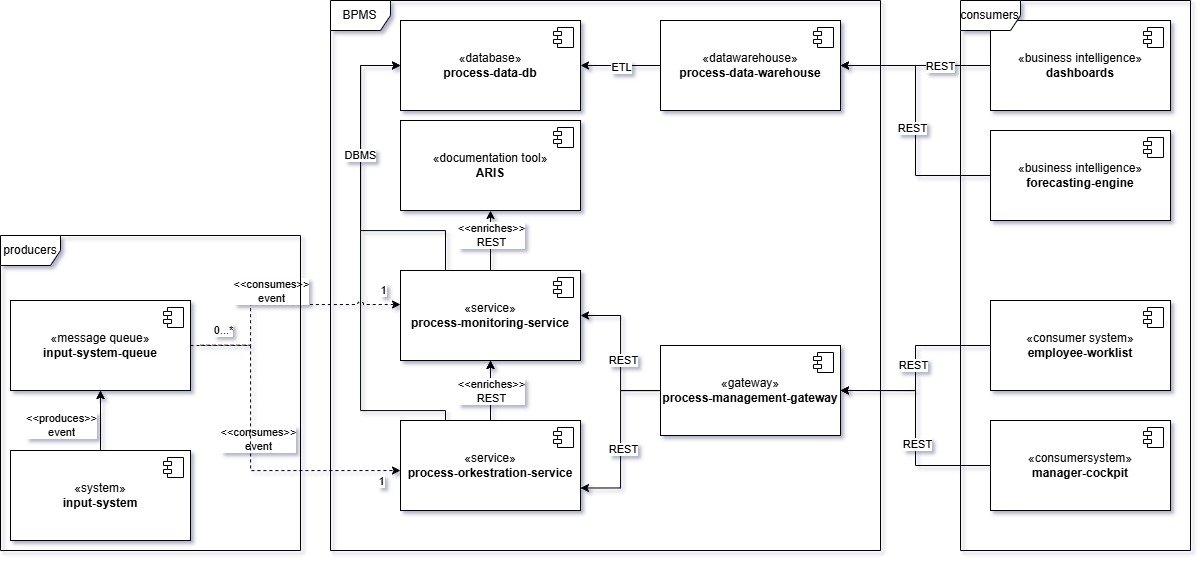
\includegraphics[width=1.0\linewidth]{theoretisch architectuur.jpg}
  \captionof{figure}[Architecturaal model van het theoretisch systeem]{Architecturaal model van het theoretisch systeem.}
\end{center}
Het theoretisch systeem volgt de microservice architectuur van het bedrijf met een duidelijke afscheiding tussen de services met een proces monitoring service en een orkestratie service als executie engine. Beide systemen krijgen hun input via eventing. Zodra de processen bepaalde mijlpalen bereiken zoals gedefinieerd in de BPMN van het proces, produceren de bijhorende systemen een event die op de queue leeft. Deze worden dan geconsumeerd door beide systemen om data rond het proces en om taken voor de medewerkers te genereren. \newline

Binnen het bedrijf wordt de proces documentatie tool ARIS gebruikt om processen te modelleren en te documenteren. Deze heeft een REST-API die het theoretisch systeem kan bevragen. Het proces monitoringsysteem bevraagt ARIS voor info over de processen om context op te bouwen indien nodig. De orkestratie gebruikt dan de monitoring voor context om zijn beslissingen te maken. Beide systemen schrijven naar dezelfde databasis met verschillende schema’s. Deze databasis wordt dan geëxtraheerd naar een datawarehouse voor datamining en business intelligence. Een gateway dient als enige punt van toegang voor externe systemen voor mediatie en extra beveiliging. Op basis van de vragen die binnenkomen op de API van de gateway bevraagt deze de correcte achterliggende systemen, ook als er meerdere instanties van de systemen draaien door horizontale opschaling. \newline

Via deze aanpak wordt een maximale ontkoppeling tussen de systemen gegarandeerd, bestaat de optie om op te schalen bij zwaardere lading op het systeem, is asynchrone dataverwerking door met een event queue te werken bereikt en bestaat de mogelijkheid voor zowel offline als online data analytische onderzoek door tegelijk te werken met een transactioneel databasis dat een historische datadimensie verkrijgt door stelselmatig te extraheren naar een datawarehouse. \newline

\subsubsection{\IfLanguageName{dutch}{Proof-of-Concept}{Proof-of-Concept}}%
\label{subsubsec:architect Proof-of-concept}
\begin{center}
  \captionsetup{type=figure}
  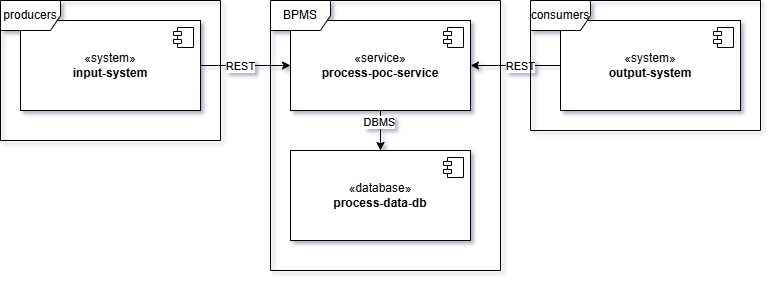
\includegraphics[width=1.0\linewidth]{poc-architectuur.jpg}
  \captionof{figure}[Architecturaal model van het proof-of-concept systeem]{Architecturaal model van het proof-of-concept systeem.}
\end{center}
Voor de proof-of-concept zal de architectuur simpeler zijn daar dit systeem enkel maar moet bewijzen dat het concept werkt. Een proof-of-concept hoort niet in te haken op de event hub, dus deze zal synchroon zijn data krijgen via zijn REST-API in plaats van asynchroon events te verwerken. Dit geeft als voordeel dat voor de tests en demo de input gesimuleerd kan worden via Postman. Monitoring en orkestratie gaan maar één specifiek proces verwerken voor de proof-of-concept waardoor een integratie met de documentatie tool van het bedrijf overbodig is. Er gaan ook geen bestaande afnemers gekoppeld worden om de werking het systeem te valideren, maar dit wordt manueel gedaan door het systeem via zijn API te bevragen. Hierdoor zijn een gateway en datawarehouse ook nodeloze complexiteit.\newline

Door in de proof-of-concept de focus te leggen op de monitor en de executie engine als de centrale componenten van het BPMS-systeem kan snel en efficiënt bewezen worden dat het systeem doet wat verwacht wordt zonder impact op de bestaande infrastructuur en met zo weinig mogelijk extra kosten voor het bedrijf zelf.

\subsection{\IfLanguageName{dutch}{Domein Model}{Domein Model}}%
\label{subsec:domein model}
Binnen het domein staan twee objecten centraal. Een proces monitoringsysteem draait rond het genereren van executie logs die gebruikt worden om de lopende processen te volgen terwijl een orkestratie systeem taken genereert voor medewerkers op het juiste moment en dit beiden op basis van de input van de externe systemen. 

\subsubsection{\IfLanguageName{dutch}{Theoretisch Systeem}{Theoretisch Systeem}}%
\label{subsubsec:domein theoretisch systeem}
\begin{center}
  \captionsetup{type=figure}
  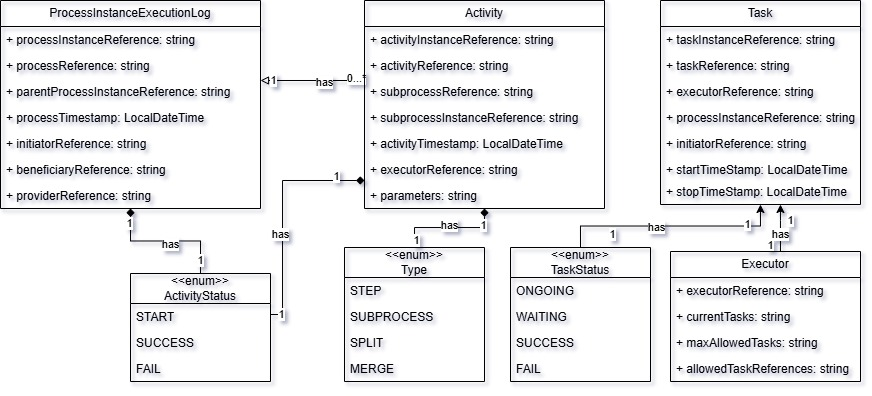
\includegraphics[width=1.0\linewidth]{theoretisch domein.jpg}
  \captionof{figure}[Domein model van het theoretisch systeem]{Domein model van het theoretisch systeem.}
\end{center}
Beide objecten worden in dit domein model opgemaakt, maar staan los van elkaar. Dit is logisch gezien monitoring en orkestratie wel samen werken en elkaar voeden, maar nooit deel uitmaken van elkaar. Bij de opmaak van het domein werden een aantal vereisten opgelegd door de systeem architect gevolgd. \newline

Enerzijds moet het systeem proces-agnostisch zijn. Dit wil zeggen dat de proces monitoring de input van om het even welk systeem en proces binnen het bedrijf moet kunnen aanvaarden en monitoring genereren. De executie logs horen ook zoveel mogelijk de BPMN-standaard te volgen om de interoperabiliteit met bestaande de documentatietool te vergemakkelijken. Een executie log van een proces kan daarom zowel de log van een proces als een sub proces zijn met referentie naar het bovenliggend proces. Een activiteit binnen de log kan een handeling binnen de BPMN-standaard als zijnde een atomair stuk werk voorstellen. Eveneens kan het een beslissing node waarop het verloop kan uitsplitsen in verschillende activiteiten en weer samenkomt voorstellen. Verder kan het ook een sub proces als deel van het bovenliggend proces voorstellen. Door te werken met de types STEP (handeling), SPLIT (uitsplitsing), MERGE (samenkomst) en SUBPROCESS (sub proces) voor elke activiteit worden deze uit elkaar gehouden. De collectie aan activiteiten die sequentieel elkaar opvolgen vormen dan het verloop van dit proces. Hierbij is het architecturaal niet de taak van het systeem om context te geven aan de ruwe data, maar wel aan de afnemer van de data. Die zal dan op basis van de data uit het monitoringsysteem en de data uit de documentatie tool een reconstructie van het procesverloop kunnen maken. \newline

Anderzijds horen zowel de taken als executie logs enkel maar referenties naar data in andere systemen te bevatten. Zodoende kan enkel maar de afnemer, die weet waar hij de juiste data op basis van de referenties moet opvragen, de data reconstrueren. Zo worden immers datalekken binnen het systeem vermeden. Dit zorgt ervoor dat zowel de executie logs als de taken vooral bestaan uit referentie id’s, tijdsvermeldingen en voorgedefinieerde statussen. Het domein bevat de volgende velden met bijhorende uitleg:
\begin{itemize}
  \item processReference: referentie naar het proces in de documentatietool.
  \item processInstanceReference: unieke referentie naar een specifieke run van het proces.
  \item parentProcessInstanceReference: Refereert naar het bovenliggend proces waarvan dit proces een stap is. Dit is enkel ingevuld als het proces een sub proces is.
  \item processStatus: de huidige status van het volledig proces zijnde START, SUCCES of FAIL.
  \item processTimestamp: de tijdsvermelding van de huidige status van het proces.
  \item initiatorReference: referentie naar het object waarvoor dit proces is opgestart. Dit is bijvoorbeeld een klant of een medewerker.
  \item beneficiaryReference: referentie naar object dat onderwerp is van het proces. Dit is bijvoorbeeld een medewerker van een klant of een factuur bij een klant.
  \item providerReference: referentie naar het systeem binnen het bedrijf die bezitter is van het proces. Het proces start en eindigt normaal in dit systeem.
  \item activityReference: referentie naar een activiteit of beslissing node of subproces in de documentatietool indien relevant.
  \item activityInstanceReference: unieke referentie naar deze specifieke run van de activiteit binnen het proces.
  \item subprocessReference: referentie naar een subproces in de documentatietool indien relevant.
  \item subprocessInstanceReference: unieke referentie naar deze specifieke run van het sub proces indien relevant.
  \item activityStatus: de huidige status van de activiteit zijnde START, SUCCES of FAIL.
  \item activityTimestamp: de tijdsvermelding van de huidige status van de activiteit.
  \item executorReference: de huidige uitvoerder van de activiteit, indien relevant. Dit kan een medewerker zijn binnen het bedrijf of een systeem.
  \item type: het soort activiteit zijnde STEP, SPLIT, MERGE of SUBPROCESS.
  \item parameters: vrij veld voor metadata.
  \item taskReference: referentie naar de taak in de documentatietool.
  \item taskInstanceReference: unieke referentie naar deze specifieke run van de taak
  \item startTimestamp: de tijdsvermelding van de start van de taak.
  \item stopTimestamp: de tijdsvermelding van de stop van de taak.
  \item taskStatus: de huidige status van de taak zijnde ONGOING, WAITING, SUCCES, FAIL.
  \item currentTasks: het aantal taken dat de betreffende executor momenteel uitvoert.
  \item maxAllowedTasks: het aantal taken dat een executor mag hebben om overwerk te voorkomen.
  \item allowedTaskReferences: een exhaustieve lijst van type taken dat deze executor mag uitvoeren op basis van zijn kennis, vaardigheden of team.
\end{itemize}
Omdat de executie logs proces-agnostisch moeten zijn, is er veel metadata nodig om te kunnen opzoeken waar in de documentatietool het proces, de activiteit of de taak hoort, van waar de data komt, wie momenteel bezig is aan een taak en voor welke klant het proces draait.  Dit is echter van vitaal belang om enerzijds de juiste data op te kunnen vragen voor de afnemers en anderzijds voor de correcte reconstructie van het verloop bij analyse en business intelligence.
\subsubsection{\IfLanguageName{dutch}{Proof-of-Concept Systeem}{Proof-of-concept Systeem}}%
\label{subsubsec:domein proof-of-concept systeem}
\begin{center}
  \captionsetup{type=figure}
  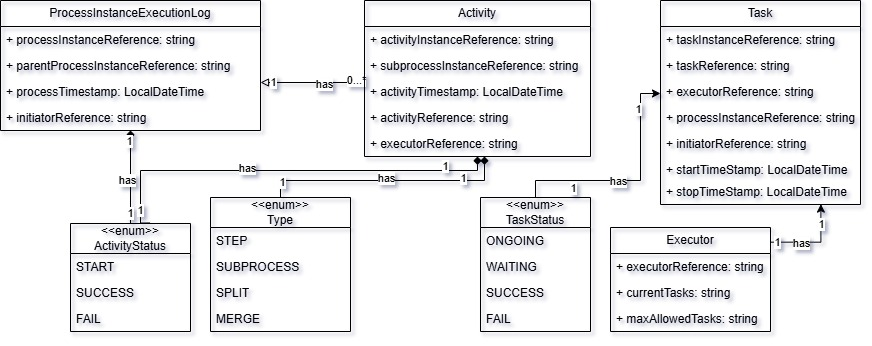
\includegraphics[width=1.0\linewidth]{poc domein.jpg}
  \captionof{figure}[Domein model van het proof-of-concept systeem]{Domein model van het proof-of-concept systeem.}
\end{center}
Gezien de proof-of-concept veel kleiner in scope is, kan het domein model ook drastisch verkleind worden. De referenties naar de documentatietool zijn verwijderd omdat de proof-of-concept niet moet kunnen integreren hiermee. De referenties naar externe systemen zijn eveneens verwijderd gezien de input gesimuleerd zal worden via Postman. Om verdere nutteloze complexiteit te mijden, kan in de proof-of-concept elke executor alle taken van het simulatie proces uitvoeren en wordt er enkel maar gekeken naar het balanceren van de werklast. Hierdoor bereikt het domein zijn minimale essentiële vorm waarbij voor een specifiek instantie van proces een executie log kan gegenereerd worden die het verloop van het proces kan representeren op een manier die strookt met de BPMN-standaard en eveneens taken kan genereren. 

\subsection{\IfLanguageName{dutch}{Entiteit Relationeel Diagram}{Entiteit relationeel diagram}}%
\label{subsec:entiteit relationeel diagram}
Het domein model wordt verder gebruikt als basis voor het entiteit relationeel diagram. Het diagram is gemaakt voor een SQL-databasis omdat het casusbedrijf aangeeft dat dit de standaard is. Voor zowel het theoretisch systeem als de proof-of-concept lijkt dit dus een correcte beslissing. Het domein model is in ieder geval compatibel met zowel SQL als een No-SQL documentstore. \newline

Gezien de aard van het systeem zou naast een SQL-databasis een documentstore ook zeker op zijn plaats zijn. Het systeem bevat immers vooral referenties naar andere systeem. Intern is er enkel een one-to-many relatie tussen de executie log van het proces en de uitgevoerde activiteiten en een one-to-one tussen taak en uitvoerder. Dit is hierdoor makkelijk te modelleren als een document waarbij de executie log een array aan activiteiten bevat. Volgens het CAP theoretisch model van Brewer is een documentstore een betere keuze voor de proces monitoring gezien de ingestie van brede data aan hoog volume hier primair is. Dit betekent dat er meer waarde is in het schalen van de databasis en in algemene bereikbaarheid van data dan in consistentie. Voor de orkestratie zou SQL echter altijd de juiste keuze zijn gezien consistente taken hebben voor de medewerkers belangrijker is dan schalen.  Bij de opzet van het theoretische systeem zou het zeker een waardevolle oefening zijn om de voordelen en nadelen van een volledig SQL-databasis versus een hybride oplossing te onderzoeken.

\subsubsection{\IfLanguageName{dutch}{Theoretisch Systeem}{Theoretisch Systeem}}%
\label{subsubsec:erd theoretisch systeem}
\begin{center}
  \captionsetup{type=figure}
  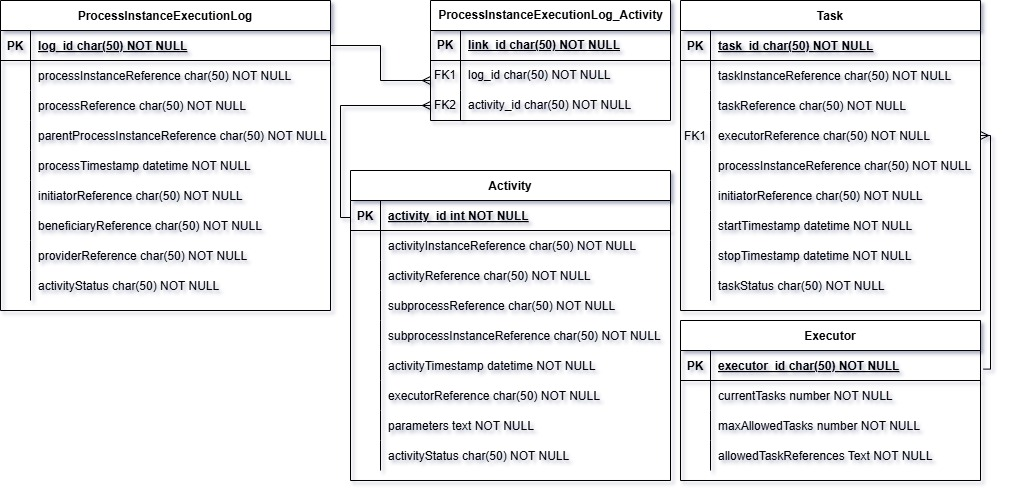
\includegraphics[width=1.0\linewidth]{theoretische ERD.jpg}
  \captionof{figure}[ERD van het theoretisch systeem]{Entiteit Relationeel Diagram van het theoretisch systeem.}
\end{center}
Dit model is opgebouwd uit vier complexe tabellen die vooral referentie data, statussen en tijdsvermeldingen bevatten. Dit volgt de redenering dat het systeem zijn eigen data niet moet kunnen interpreteren en dit moet overlaten aan andere systemen. De executie log heeft een one-to-many relatie met zijn activiteiten via een tussentabel terwijl taken een one-to-one relatie heeft met zijn uitvoerder. Dit is nodig zodat het systeem taken aan de correcte medewerkers qua werklast en toegelaten taken kan uitdelen. Het systeem moet dus een simpele subset reflectie bevatten van de master data omtrent wie welke taken mag uitvoeren en bijhouden hoeveel taken deze mensen momenteel uitvoeren versus hun maximaal toegelaten lading.

\subsubsection{\IfLanguageName{dutch}{Proof-of-Concept Systeem}{Proof-of-concept Systeem}}%
\label{subsubsec:erd proof-of-concept systeem}
\begin{center}
  \captionsetup{type=figure}
  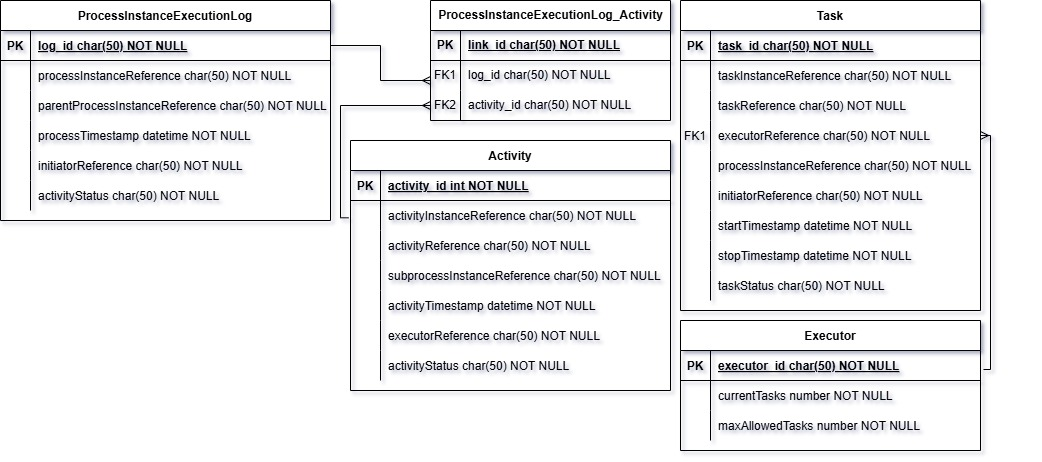
\includegraphics[width=1.0\linewidth]{poc erd.jpg}
  \captionof{figure}[ERD van het proof-of-concept systeem]{Entiteit relationeel diagram van het proof-of-concept systeem.}
\end{center}
Het diagram voor de proof-of-concept volgt dezelfde structuur als die van het theoretisch systeem, maar is uiteraard versimpeld door de kleinere scope van het systeem. Dezelfde informatie die in het domein model wordt weggelaten is hier ook afwezig.

\subsection{\IfLanguageName{dutch}{REST-API}{REST-API}}%
\label{subsec:rest-api}
De technische vereisten van het casusbedrijf vereisen een duidelijke en veilige API voor afname van data. Dit omdat het in eerste instantie niet gewenst is dat een eindgebruiker of extern systeem rechtstreeks kan ingrijpen op de generatie van executie logs of taken. In een latere iteratie van het systeem zal dit echter wel nodig zijn omdat business aangaf dat de optie er moet zijn om expliciet in te grijpen op taken door bepaalde dossiers voorrang te geven of om taken rechtstreeks toe te wijzen aan specifieke medewerkers. 

\subsubsection{\IfLanguageName{dutch}{Theoretisch Systeem}{Theoretisch Systeem}}%
\label{subsubsec:api theoretisch systeem}

Het theoretisch systeem heeft geen nood aan een API om data te ontvangen. De data zal immers komen vanuit een event of message op een hub of broker waar de data leeft tot het systeem de data consumeert. Zowel de data rond het afwerken van stappen in het proces als die van taken zal zo het systeem bereiken. Het architecturaal principe dat systemen zoveel mogelijk met elkaar moeten communiceren via events en messages als ze niet in elkaars domein zitten blijft behouden. Proces monitoring en orkestratie kan immers door zijn doel enkel deel uitmaken van zijn eigen domein. \newline

Voor afname zal er vooral nood zijn aan lees eindpunten met specifieke gelaagdheid rond de data objecten, maar ook aan export eindpunten voor extractie richting de datawarehouse.
 
\begin{center}
  \captionsetup{type=figure}
  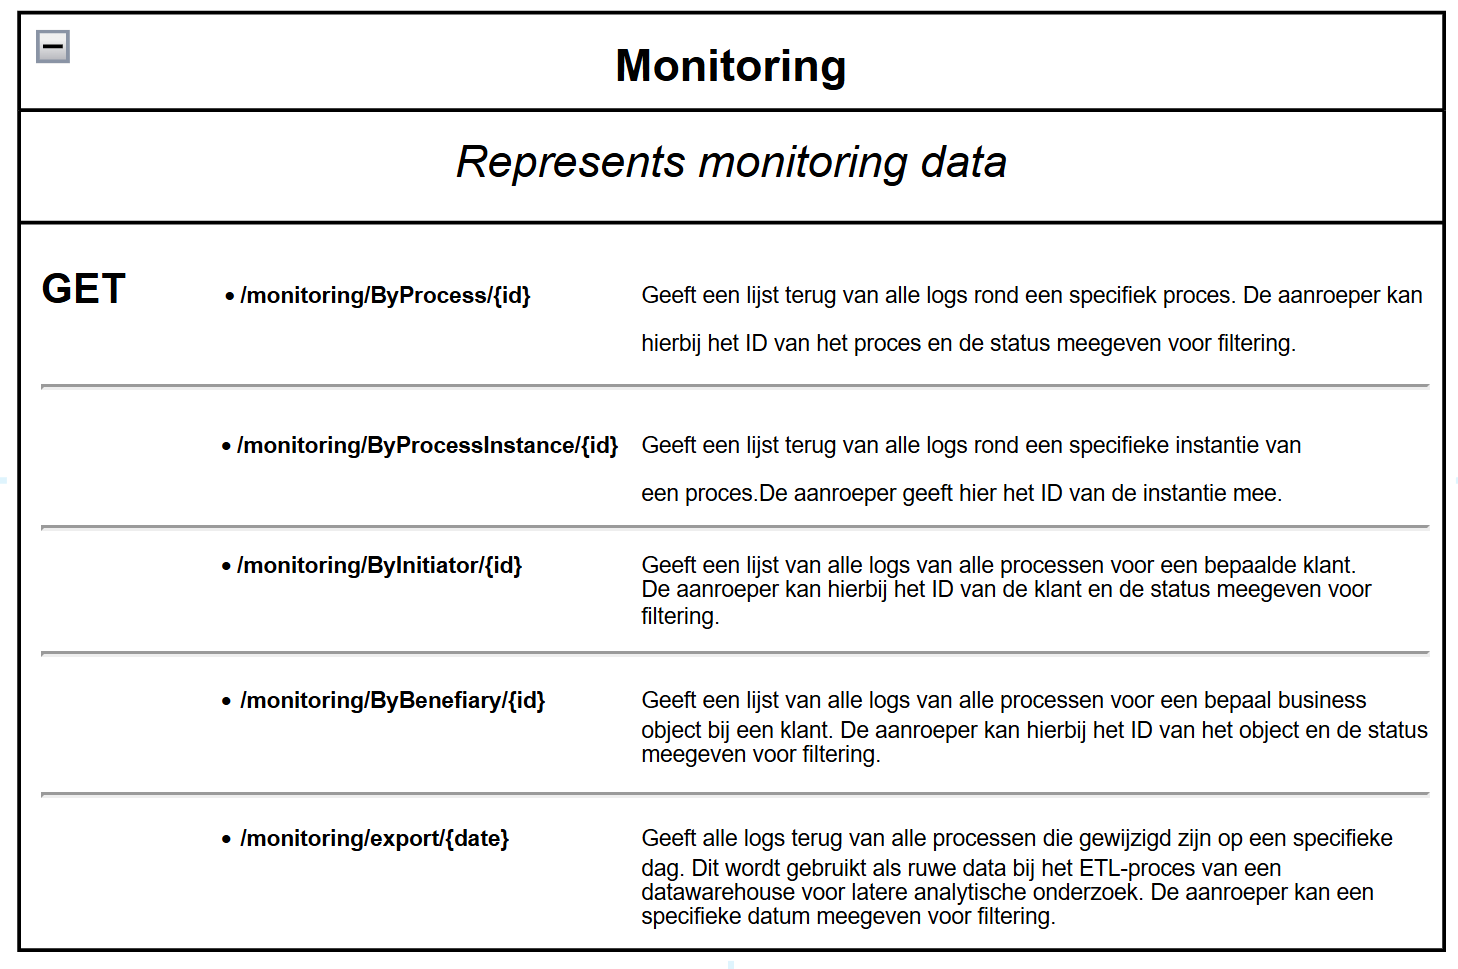
\includegraphics[width=1.0\linewidth]{theoretisch monitoring api.png}
  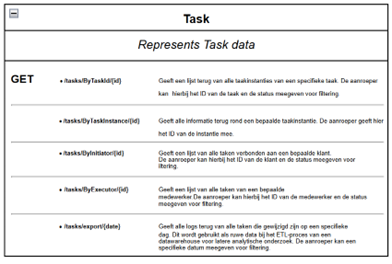
\includegraphics[width=1.0\linewidth]{theoretisch task api.png}
  \captionof{figure}[API-diagram van het theoretisch systeem]{API-diagram van het theoretisch systeem.}
\end{center}

\subsubsection{\IfLanguageName{dutch}{Proof-of-Concept Systeem}{Proof-of-Concept Systeem}}%
\label{subsubsec:api proof-of-concept systeem}
De proof of concept volgt een heel gelijkaardig stramien aan het theoretisch systeem voor afname. Door zijn gelimiteerde scope zijn de eindpunten die te maken hebben met filtering op specifieke processen en business objecten weggelaten gezien er maar één proces zonder gelaagdheid aan business items gevolgd zal worden. De eindpunten voor extractie richting de datawarehouse zijn bijgevolg ook overbodig. Omdat de proof-of-concept zijn input zal krijgen via simulatie zal deze wel eindpunten hebben waar simulatieberichten aankomen met dezelfde inhoud als de messages die het theoretisch systeem zal gebruiken. Er is ook een eindpunt voorzien die ons toelaat om bepaalde taken te markeren als voltooid of wachtende opdat we het taakoverzicht correct kunnen testen.
 
 
\begin{center}
  \captionsetup{type=figure}
  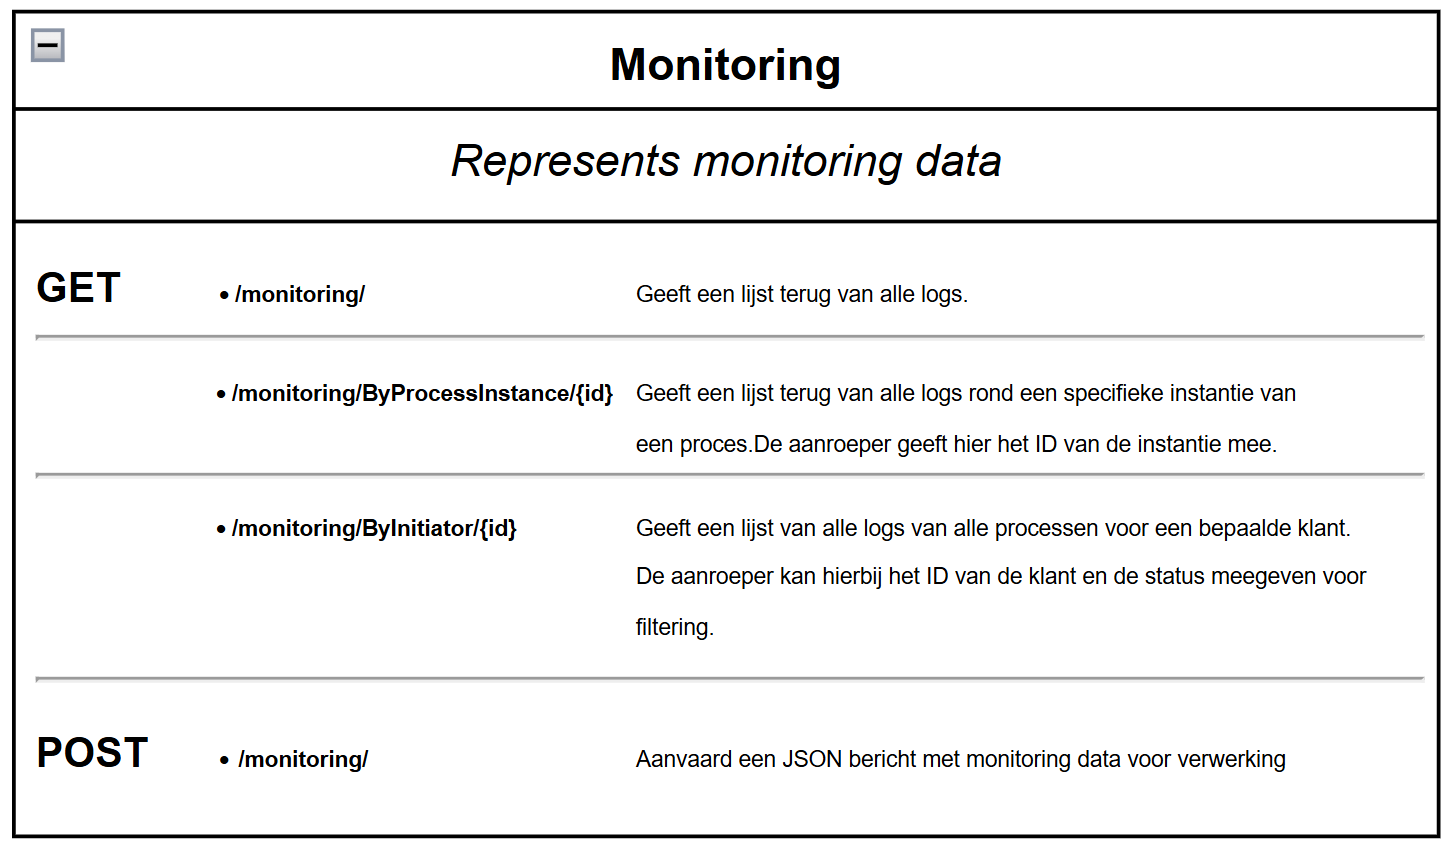
\includegraphics[width=1.0\linewidth]{poc monitoring api.png}
  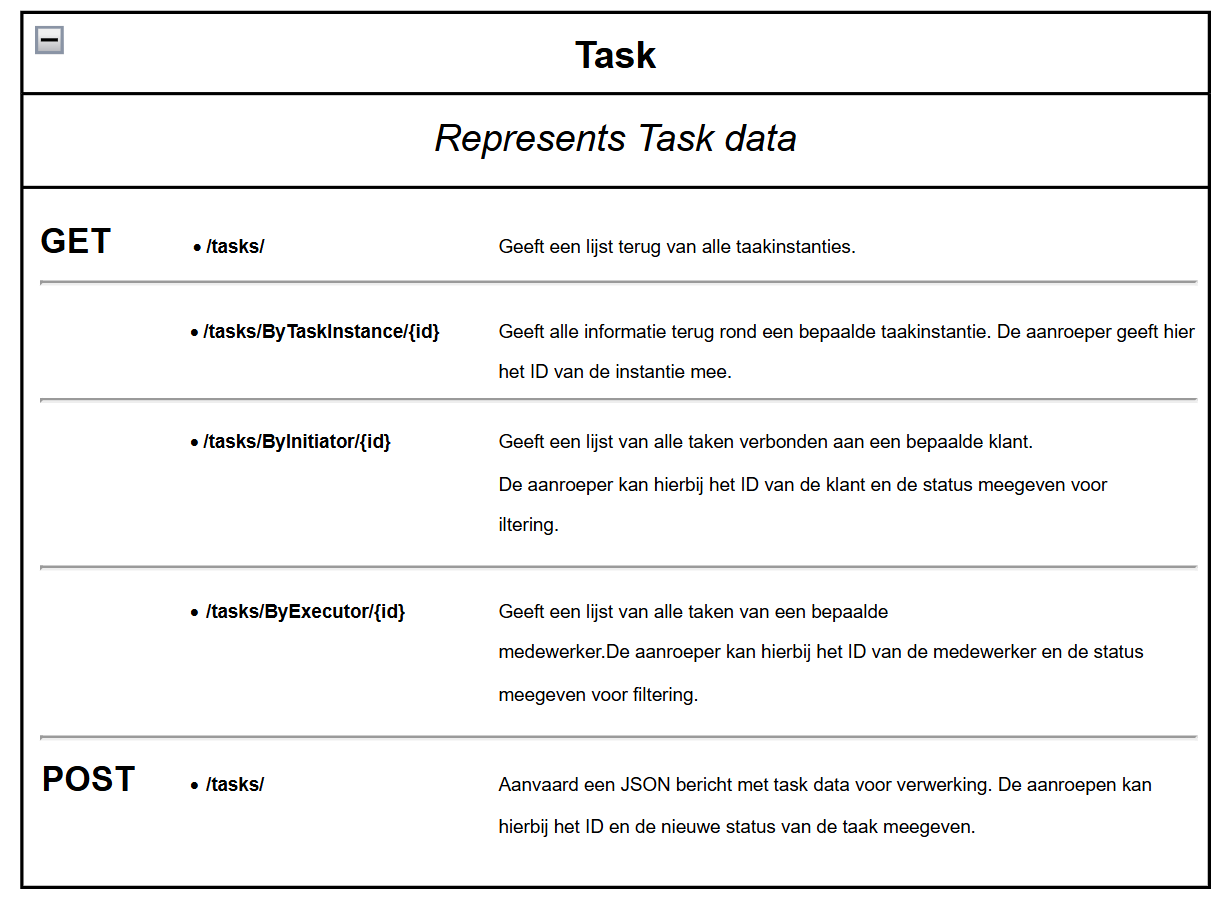
\includegraphics[width=1.0\linewidth]{poc task api.png}
  \captionof{figure}[API-diagram van het proof-of-concept systeem]{API-diagram van het proof-of-concept systeem.}
\end{center}
\section{\IfLanguageName{dutch}{Implementatie}{Implementatie}}%
\label{sec:implementatie}
Spring Boot is gemaakt voor snelle prototyping van microservices en REST-API’s waardoor het bouwproces zeer pijnloos was. De mogelijkheid om een in-memory databasis te gebruiken biedt dan ook extra voordelen voor het bedrijf gezien er geen nodeloze infrastructuur opgezet moet worden voor een aparte databasis die nadien toch verwijderd wordt.\newline

Het monitoring domein was door de gemaakte analyse betrekkelijk eenvoudig te implementeren. Het gros van de logica dient om de ruwe monitoring data te valideren en correct te interpreteren om de executielog per procesinstantie stelselmatig op te bouwen. Het moet daarom vooral in staat zijn om snel en consistent data te verwerken met oog op foutbestendigheid en correcte logging. Door de context van de data af te schermen van het systeem en de interpretatie hiervan over te laten aan de afnemer kan het systeem zijn focus leggen op zijn singuliere verantwoordelijkheid als verwerker van grote hoeveelheden aan data. \newline

Het taak domein definiëren en correct taken laten generen ging door de analyse ook zeer vlot. De grootste uitdaging was het correct inregelen van de executie engine. Bij out-of-box systemen waarbij de modelering tool rechtstreeks vasthangt aan het monitoringsysteem en de executie engine wordt de mapping tussen taak en activiteit gedaan tijdens het modelleren van het proces. Bij deze microservice aanpak waarbij de modelering tool apart blijft, moet deze mapping expliciet gedaan worden in de configuratie. Dit bleek vrij uitdagend gezien er naast een BPMN-diagram van het te simuleren proces ook een mapping moest zijn van de berichten die per milestone gingen gestuurd worden en welke taken deze potentieel kunnen genereren. Dit was nodig voor de uiteindelijke mapping van monitoring data richting taken om zo de executie engine in te regelen. \newline

Het systeem moest ook minimale kennis hebben over alle medewerkers en het aantal die ze mogen uitvoeren. Het systeem kan zo bijhouden hoeveel actieve taken een medewerker heeft om zo de werklast aan taken evenredig te verdelen. Dit werd opgelost door dummy data te injecteren in de in-memory databasis en logica te schrijven voor deze werklast balancerende werking. Deze twee elementen zorgden voor een verrassende extra laag aan complexiteit.

 \begin{center}
  \captionsetup{type=figure}
  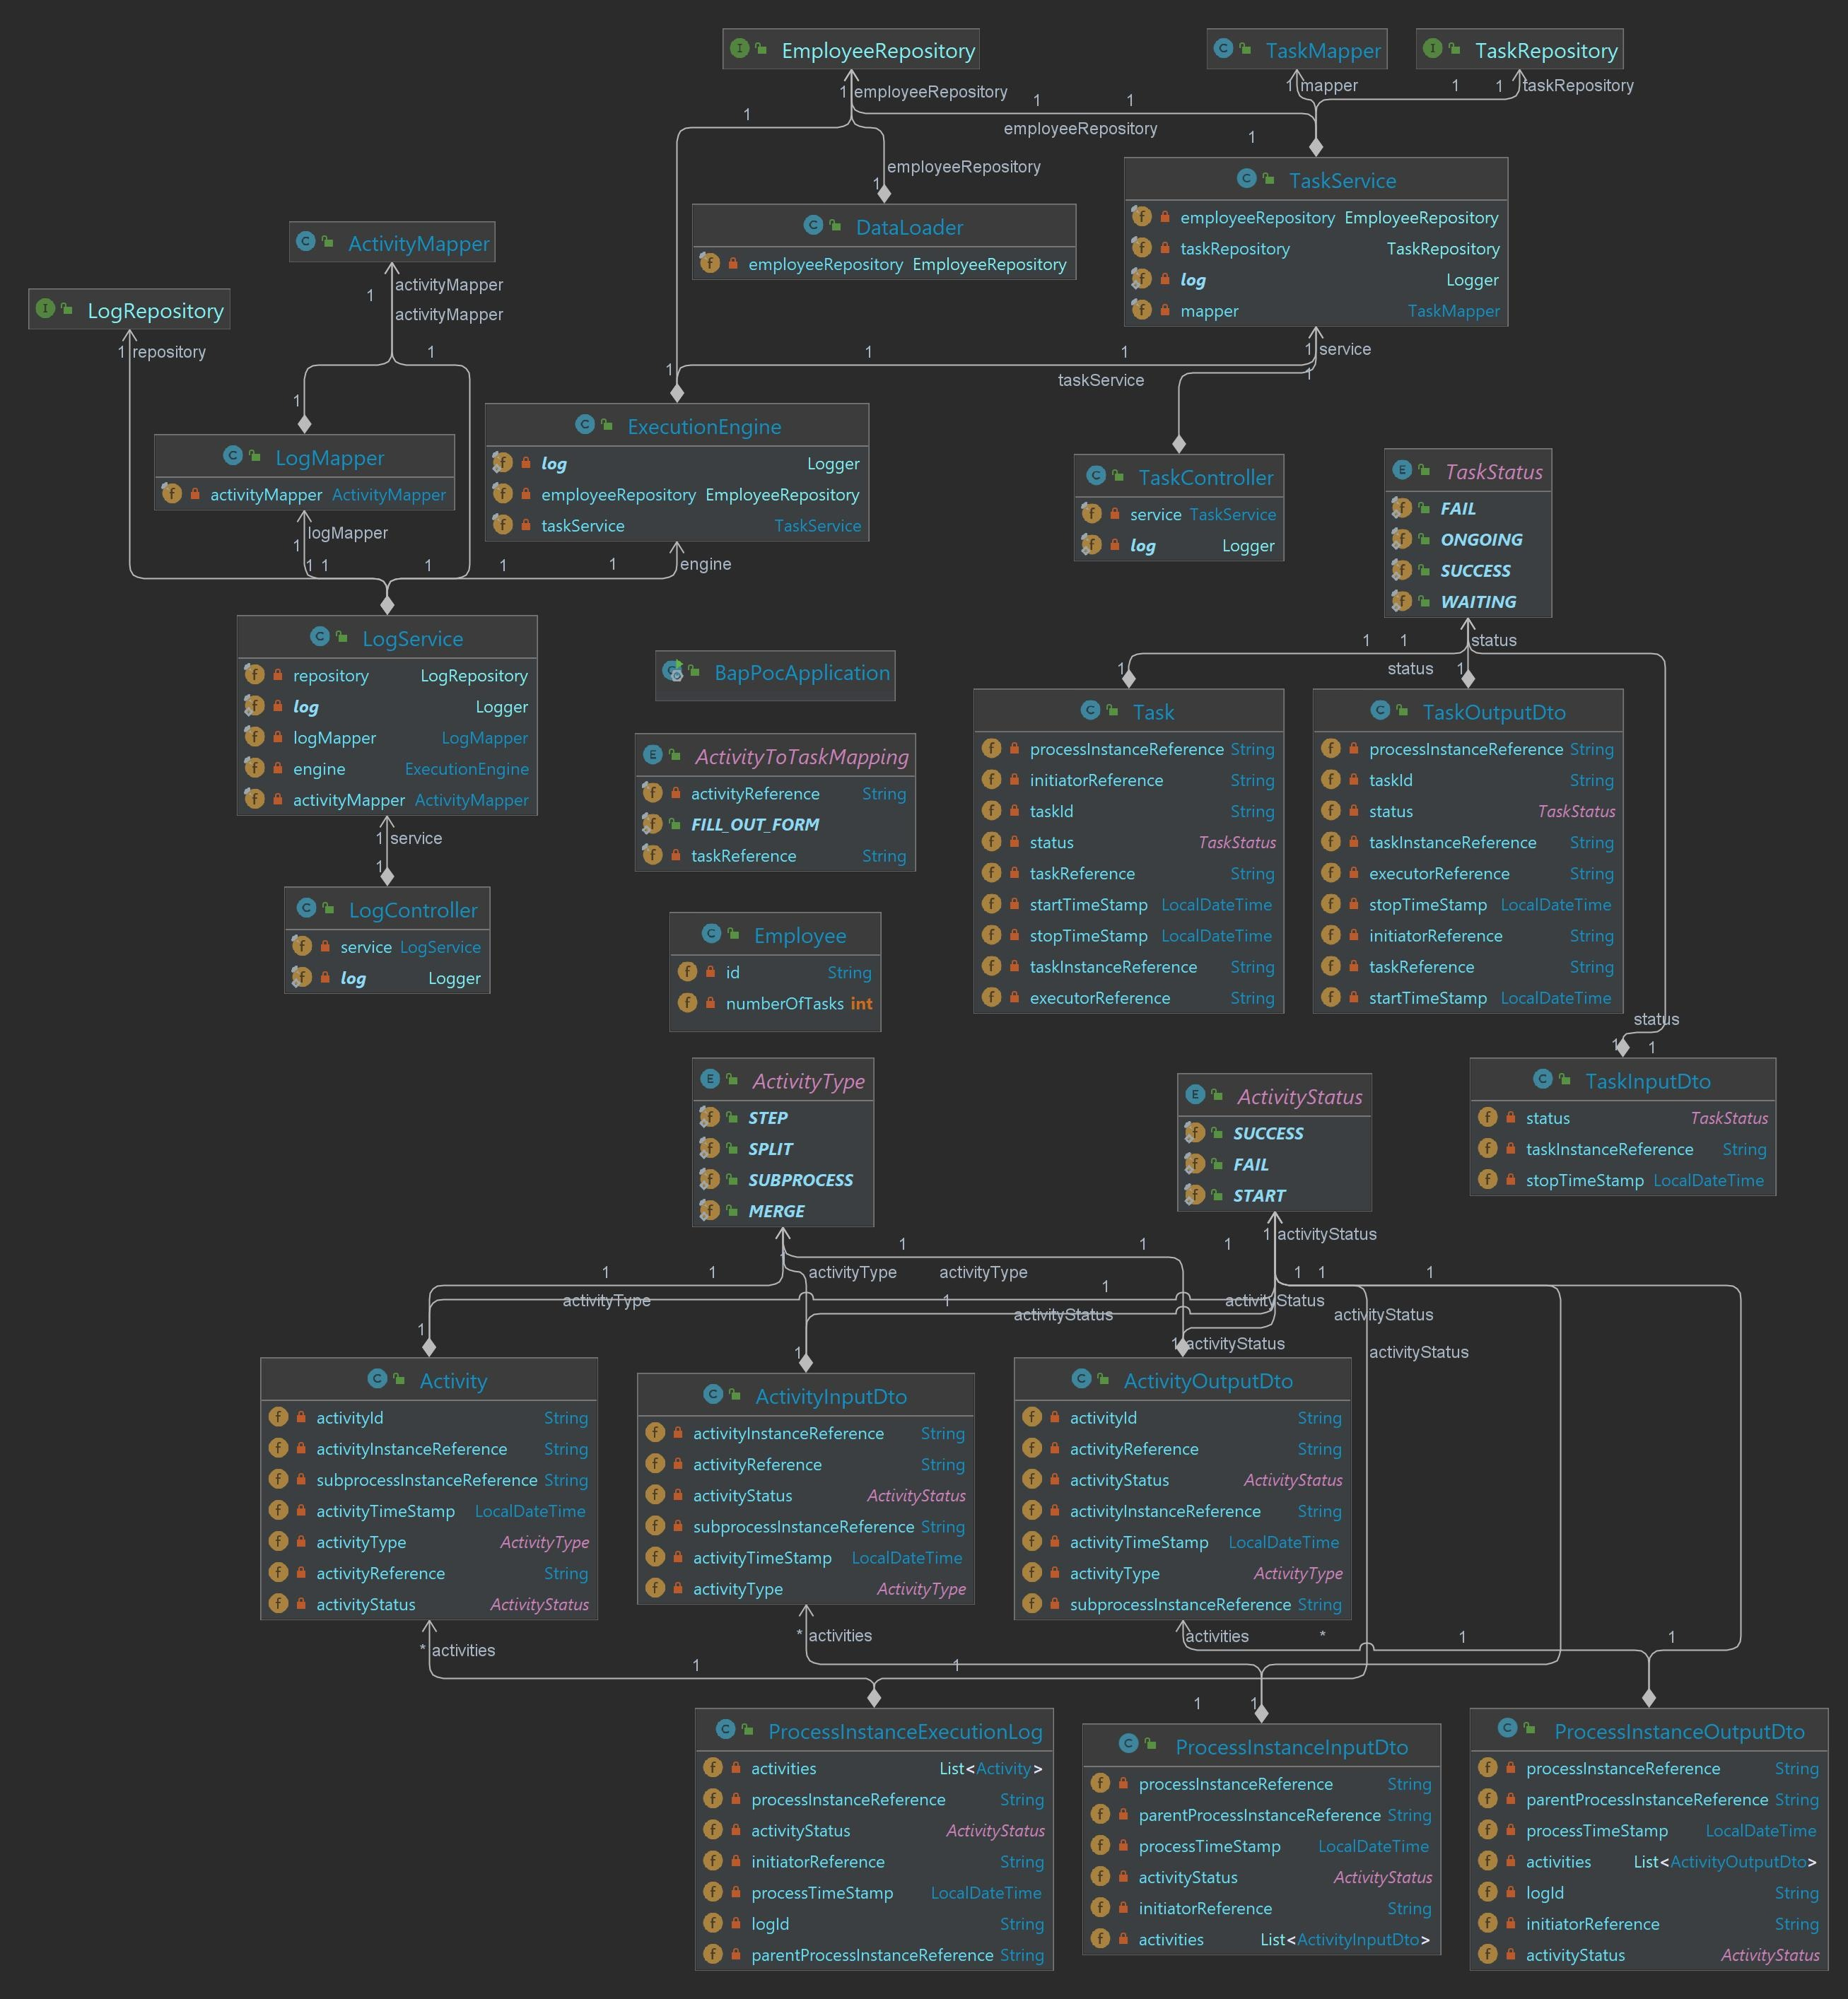
\includegraphics[width=1.0\linewidth]{product uml crop.JPG}
  \captionof{figure}[UML klasse-diagram van het proof-of-concept systeem]{UML klasse-diagram van het proof-of-concept systeem.}
\end{center}

\section{\IfLanguageName{dutch}{Validatie}{Validatie}}%
\label{sec:validatie}
Om te valideren of het systeem werkt, wordt het verloop van een bestaand proces binnen het casusbedrijf gesimuleerd. Hierbij komen via de REST-API berichten aan bij de proof-of-concept systeem die gelijkaardig zijn aan de monitoring events die het theoretisch systeem zal verwerken. Op basis van deze data moet het systeem in staat om de data van het lopend proces correct te bundelen, bloot te stellen aan afnemers en niet enkel taken te generen, maar deze ook toe te wijzen aan onze dummy medewerkers.

\begin{center}
  \captionsetup{type=figure}
  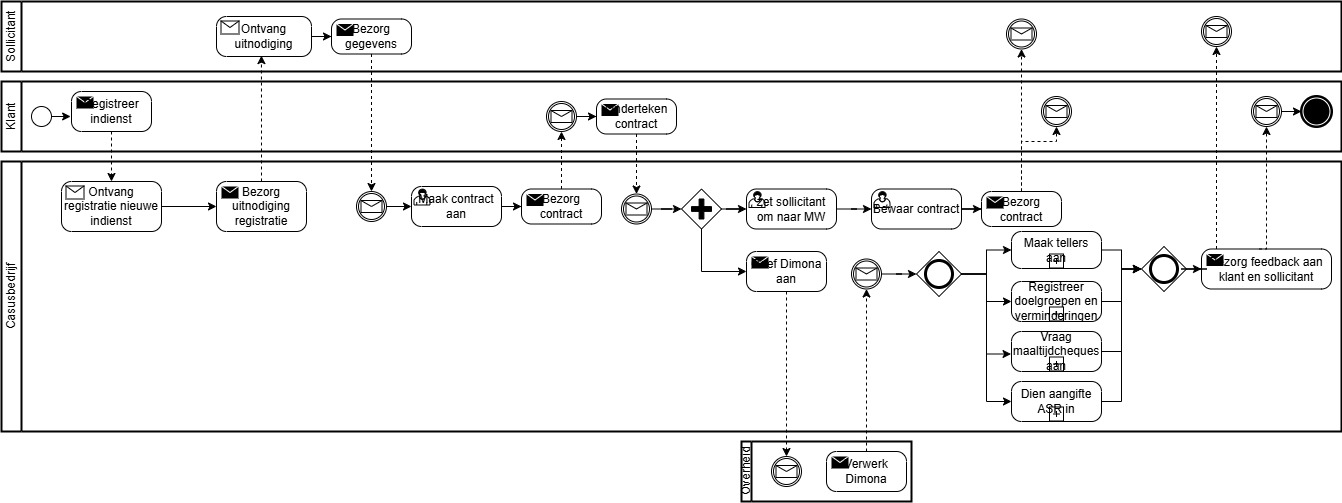
\includegraphics[width=1.0\linewidth]{test proces.jpg}
  \captionof{figure}[BPMN-diagram van het gesimuleerd intern proces]{BPMN-diagram van het gesimuleerd intern proces.}
\end{center}

Om deze validatie correct te laten verlopen werd bij elke node binnen het diagram een mapping gemaakt waarbij wordt gedefinieerd welk monitoring data dat het systeem zal ontvangen binnen de simulatie en welke taak, indien relevant, dient genereerd te worden vanuit het systeem.  Op basis hiervan werd de simulatie data opgebouwd en werd nagegaan de resulterende executielog en de gegenereerde taken voldoen aan de vereisten van het bedrijf om te valideren of de proof-of-concept succesvol is. Om de validatie te vergemakkelijken werd ook een rudimentair front-end gebouwd voor visualisaties.

\begin{center}
  \captionsetup{type=figure}
  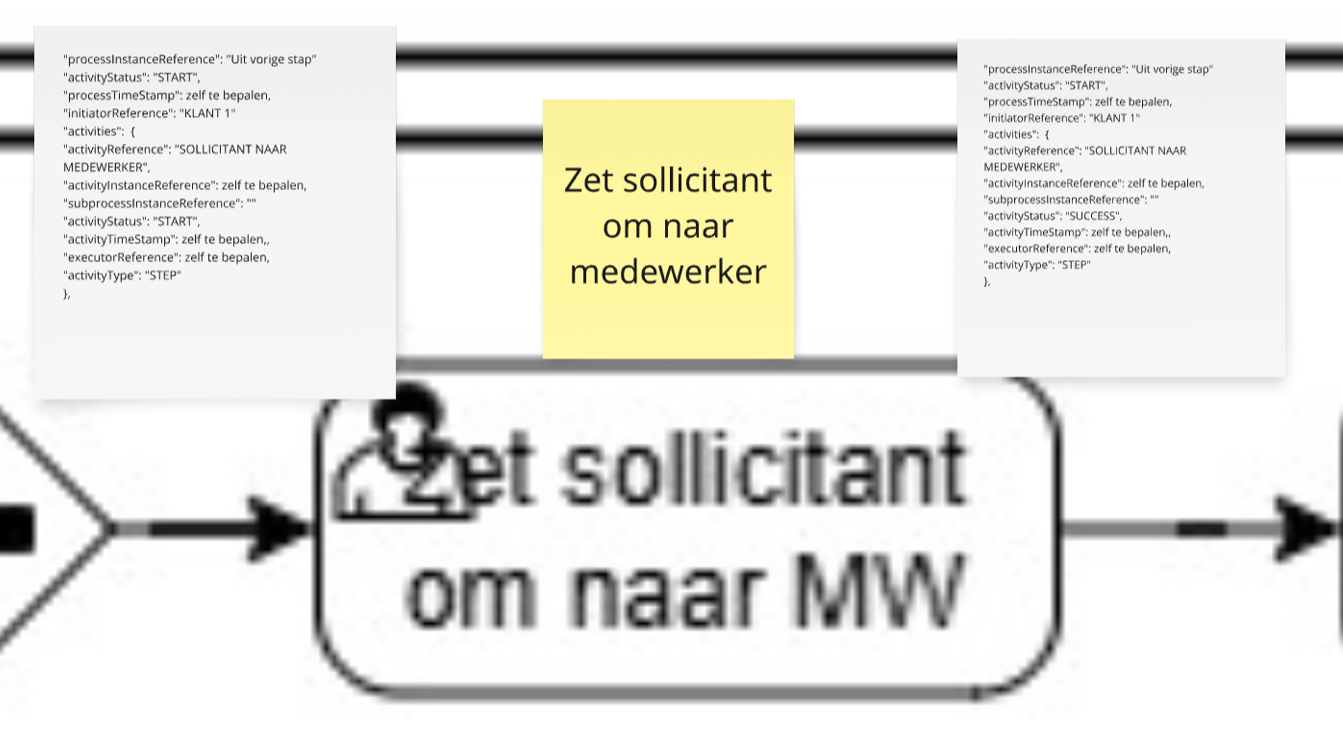
\includegraphics[width=1.0\linewidth]{node bpmn.png}
  \captionof{figure}[BPMN-node met mapping]{Een node uit het diagram met bijhorende simulatie data en verwachtte taak.}
\end{center}
 
\begin{center}
  \captionsetup{type=figure}
  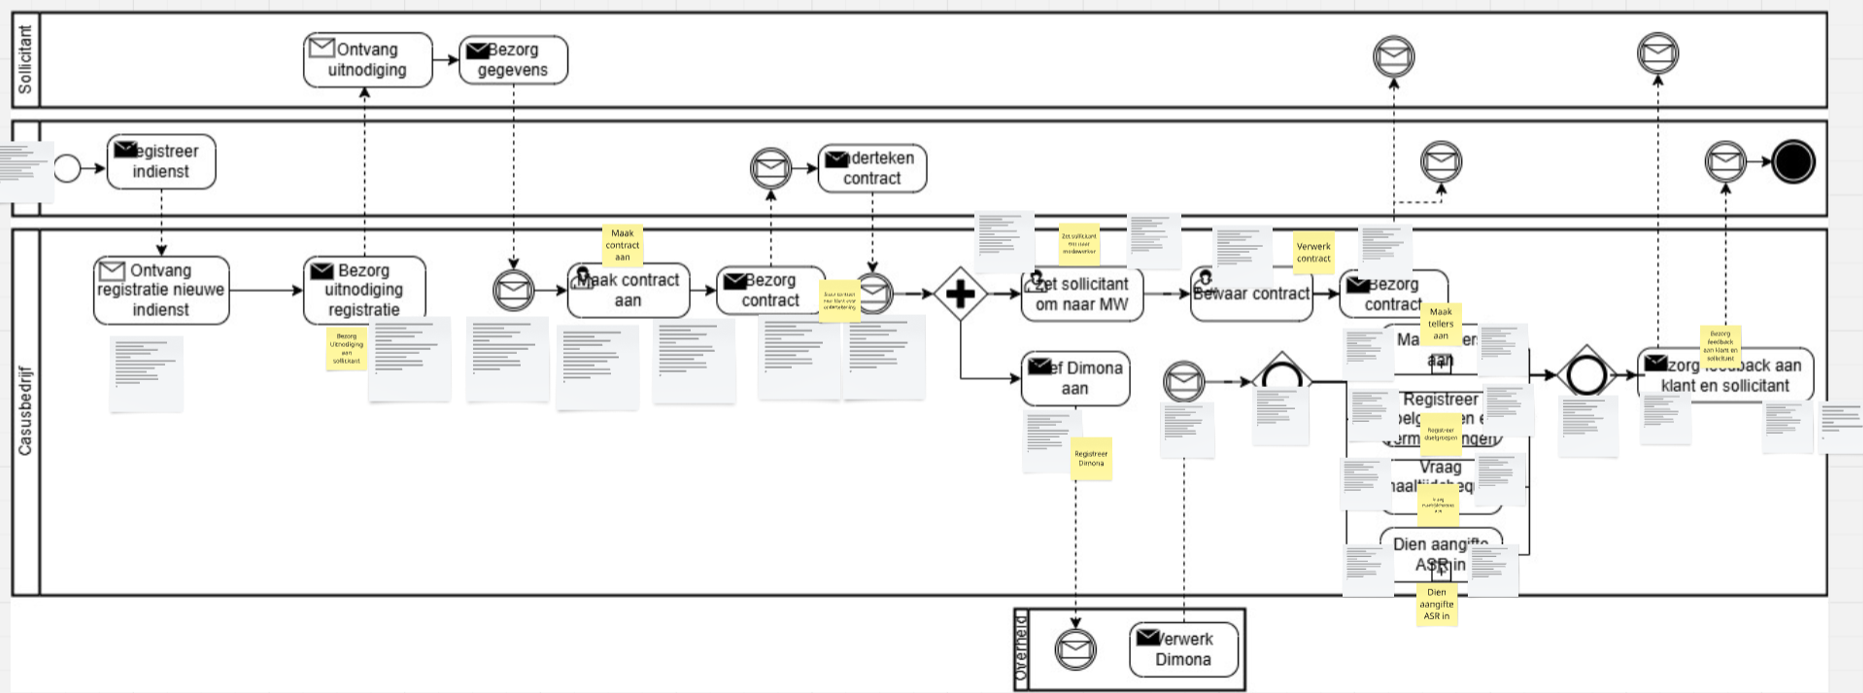
\includegraphics[width=1.0\linewidth]{bpmn met mapping.png}
  \captionof{figure}[BPMN-diagram met mapping]{Het volledig diagram met bijhorende simulatie data en verwachtte taken per node.}
\end{center}

\begin{center}
  \captionsetup{type=figure}
  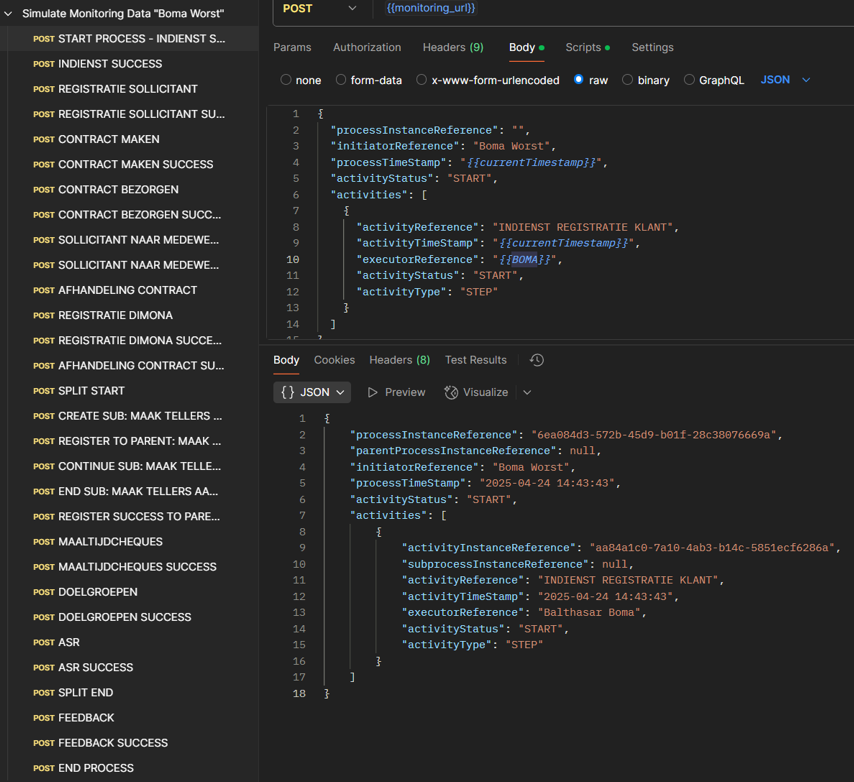
\includegraphics[width=1.0\linewidth]{postman data.png}
  \captionof{figure}[Simulatie-data Postman]{Simulatieflow voor data vanuit externe systemen in Postman.}
\end{center}
Bij aankomst van de initiële monitoring data maakt het systeem een Proces Instantie Executie Log aan die de algemene data van het proces bevat zoals zijn unieke referentie, wie het proces heeft gestart en de huidige status. De Log bevat ook een collectie aan activiteiten die het verloop van het proces sequentieel voorstelt. Zodra er nieuwe data binnenkomt, zal het systeem deze correct interpreteren, mappen in de juiste vorm en toevoegen aan de collectie. De activiteiten volgen de BPMN-standaard door gebruik te maken van de types STEP, SPLIT, MERGE en SUBPROCES. \newline

Als een activiteit ook een sub proces start, dan worden die bi-directioneel aan elkaar gekoppeld. 
\begin{center}
  \captionsetup{type=figure}
  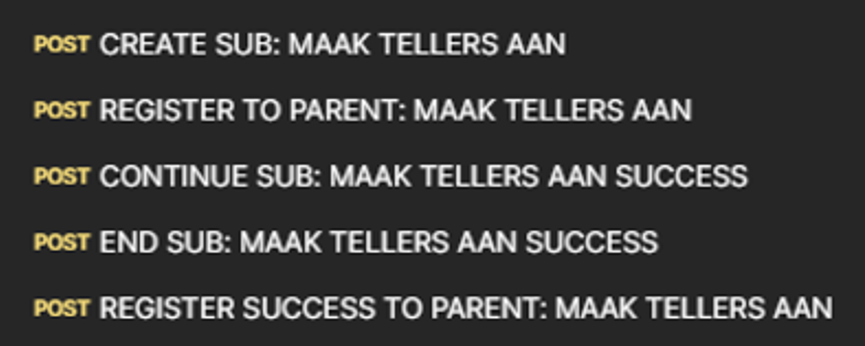
\includegraphics[width=0.75\linewidth]{postman subproces.png}
  \captionof{figure}[Subproces registratie data]{Start, koppeling aan ouder, afloop en registratie van resultaat bij sub en ouder proces.}
\end{center}
Deze data kan dan opgevraagd worden door de afnemers via een API voor implementatie in hun applicaties. In onderstaande data is zichtbaar hoe de uitvoerder een in dienst begon te registreren om 15:55 en klaar was om 16:05. Deze data kan gebruikt worden om de status van het proces terug te koppelen aan de klant, om de gemiddelde doorlooptijd van deze activiteit te berekenen of om anomalie of bottleneck detectie uit te voeren op basis van servicelevel akkoorden. 
\begin{center}
  \captionsetup{type=figure}
  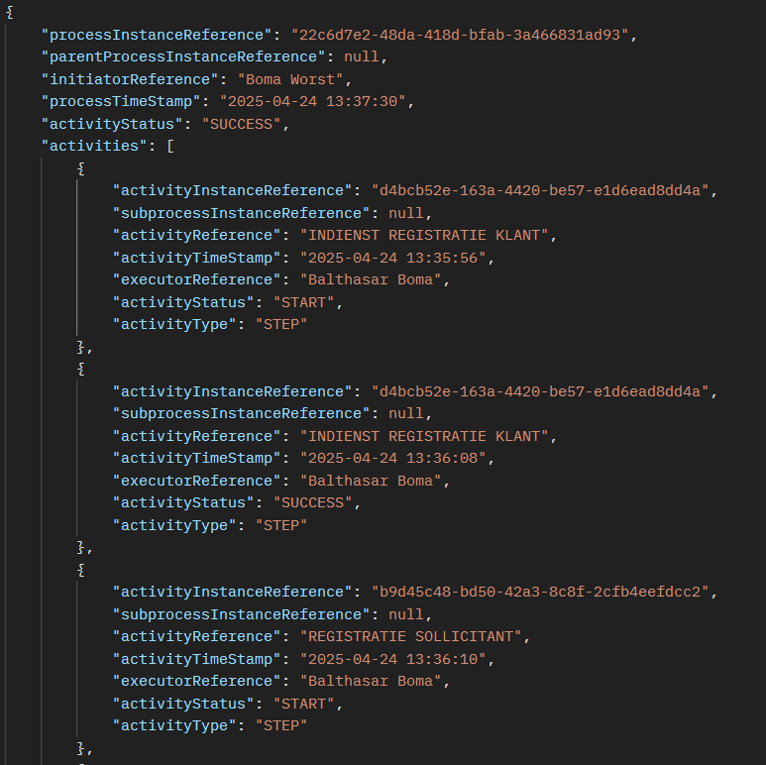
\includegraphics[width=1.0\linewidth]{JSON output api.png}
  \captionof{figure}[JSON-output API Monitoring]{JSON-output van het test-proces indien opgevraagd via de API.}
\end{center}
 
Het systeem is tevens ook in staat om een gepaste taak te genereren op het juiste moment en deze te koppelen aan een gepaste medewerker. Het weet hoeveel taken iedereen heeft en kan daardoor aan load balanceren doen. Dit is ook makkelijk op te vragen via de API.\newline

In onderstaande data zien we hoe als reactie op de activiteiten “REGISTRATIE SOLLICITANT”, “CONTRACT MAKEN” en “CONTRACT BEZORGEN” er drie verschillende taken met eigen traceerbare referenties gemaakt zijn en verbonden werden aan drie unieke medewerkers.
\begin{center}
  \captionsetup{type=figure}
  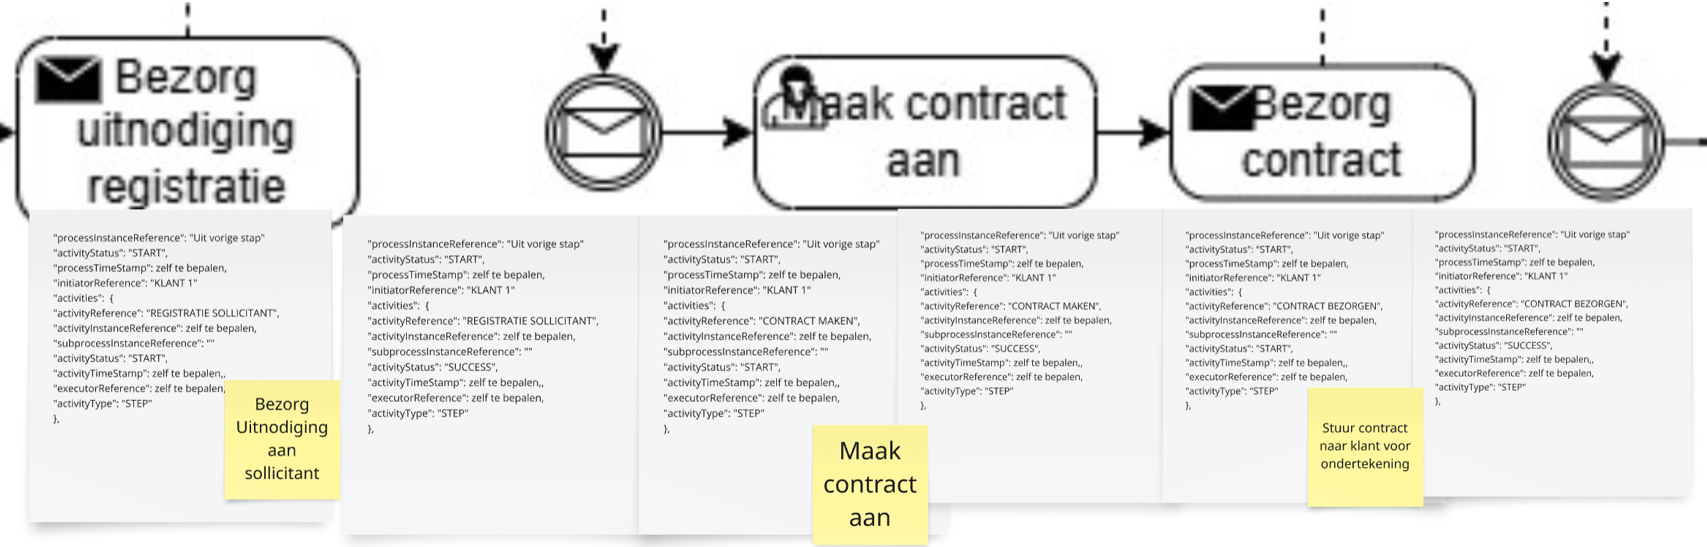
\includegraphics[width=1.0\linewidth]{nodes met taken.png}
  \captionof{figure}[Nodes met taken]{De relevante nodes uit het diagram met bijhorende simulatie data en verwachtte taken.}
\end{center}
\begin{center}
  \captionsetup{type=figure}
  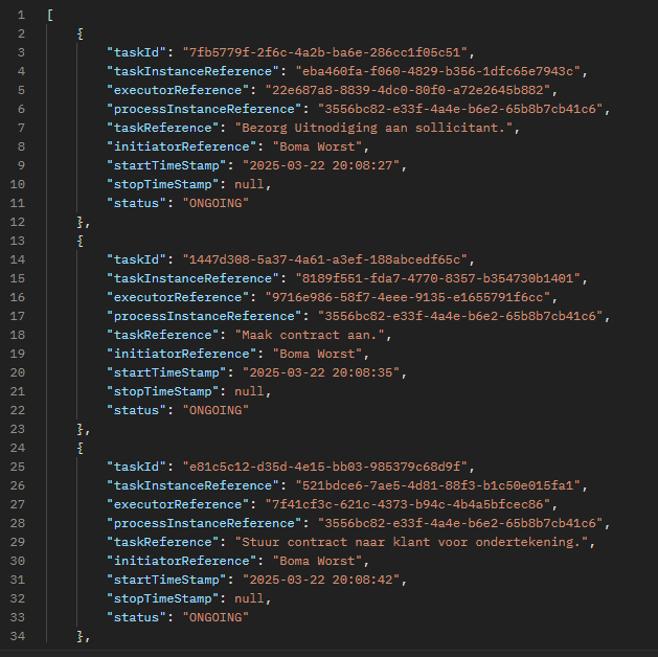
\includegraphics[width=1.0\linewidth]{taken.png}
  \captionof{figure}[SON-output API Orkestratie]{JSON-output van de drie verwachte gegenereerde taken gekoppeld aan drie verschillende medewerkers.}
\end{center}
\section{\IfLanguageName{dutch}{Visualisatie van Mogelijke Realisaties voor het Casusbedrijf}{Visualisatie van mogelijke realisaties voor het casusbedrijf}}%
\label{sec:visualisatie}
Op basis van de data die uit de API van de applicatie komt, werden rudimentaire front-end visualisaties gebouwd om te valideren of de use-cases die business in de analyse aanhaalde nu technisch mogelijk zijn. \newline

Op basis van de data in de executie logs binnen het systeem is het mogelijk om voor elke lopende instantie van het proces een tijdslijn op te bouwen. Zodoende kan de klant geïnformeerd worden over het verloop en de huidige status van het proces. \newline

Gezien elke activiteit ook oproepbaar is op basis van zijn activiteit referentie en instantie referentie is het mogelijk om alle instantie logs van een specifieke type activiteit op te roepen, de doorlooptijd per instantie te berekenen en statistisch onderzoek te plegen naar doorlooptijden of anomaliedetectie te doen.
\begin{center}
  \captionsetup{type=figure}
  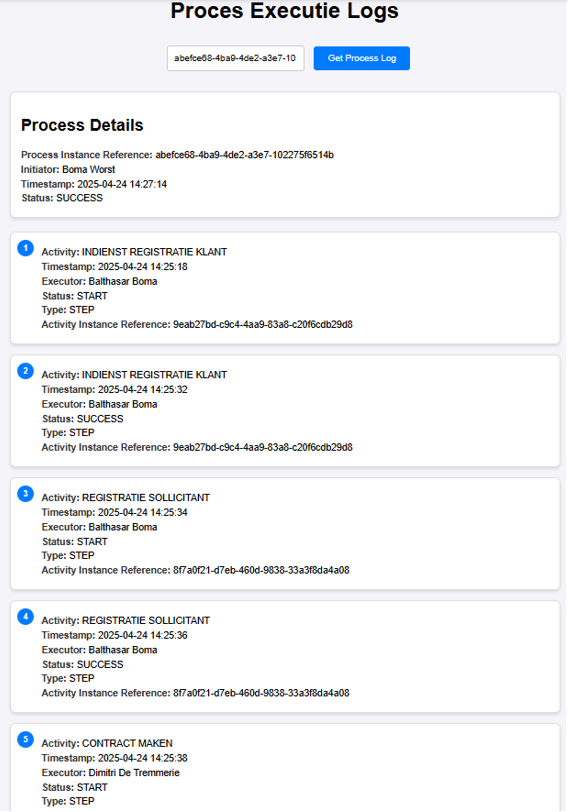
\includegraphics[width=0.89\linewidth]{timeline proces.png}
  \captionof{figure}[Executie log timeline]{Timeline van de lopende instantie van proces abefce68-4ba9-4de2-a3e7-102275f6514b met diens activiteiten in chronologische volgorde.}
\end{center}

Eerder werd de eis gesteld dat het systeem correct moet omgaan met het splitsen van de timeline in parallelle of alternatieve flows. Uit de visualisatie is duidelijk dat hier een SPLIT gebeurd in verschillende parallelle activiteiten die dan later weer samenkomt. Door de data zo te segmenteren is het mogelijk om statistisch onderzoek te doen naar bottlenecks in gesplitste flows.

\begin{center}
  \captionsetup{type=figure}
  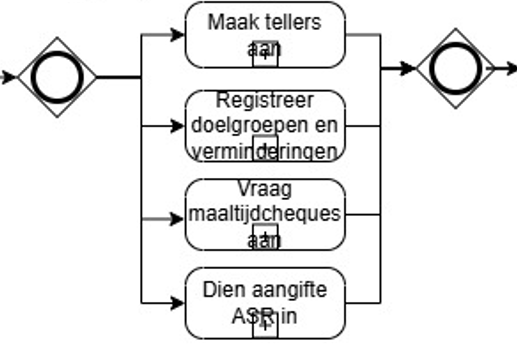
\includegraphics[width=0.75\linewidth]{upstream split.png}
  \captionof{figure}[BPMN-diagram upstream split]{Upstream split volgens het BPMN-diagram.}
\end{center}

 
\begin{center}
  \captionsetup{type=figure}
  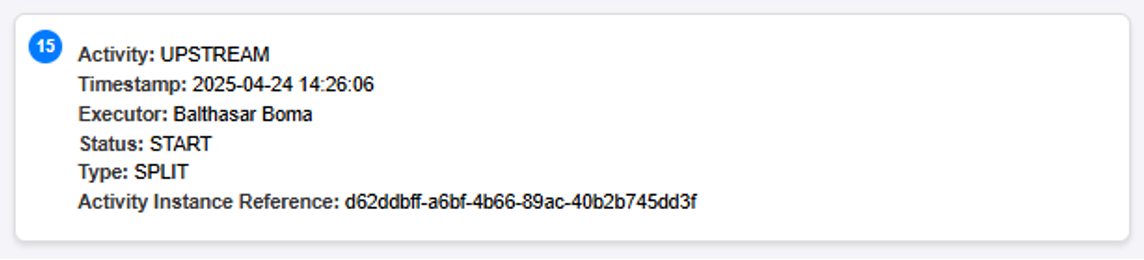
\includegraphics[width=1.0\linewidth]{upstream visual 1.png}
  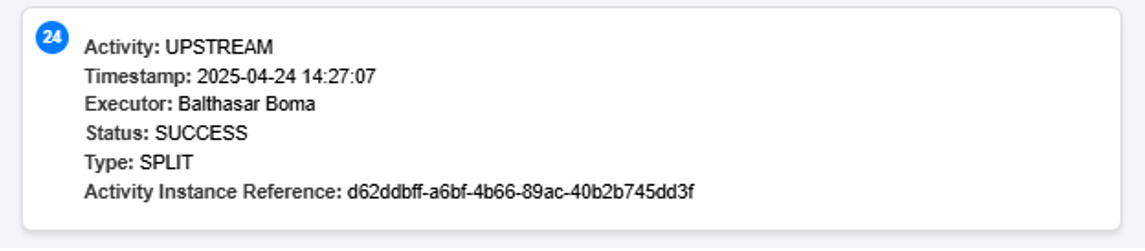
\includegraphics[width=1.0\linewidth]{upstream visual 2.png}
  \captionof{figure}[Upstream split visualisatie]{Start en stop van de split als 15de en 24ste stap in de timeline die doorlooptijd van de split berekenbaar maakt.}
\end{center}

Tijdens de split worden er ook sub processen gestart als deel van de activiteiten. Het systeem kan dit correct interpreteren, de processen starten en deze koppelen aan het bovenliggend proces om makkelijke navigatie van de data mogelijk te maken. Volgens bovenstaande BPMN-diagram is de activiteit “MAAK TELLERS AAN” een sub proces. Dit is correct gereflecteerd in de tijdslijn.

\begin{center}
  \captionsetup{type=figure}
  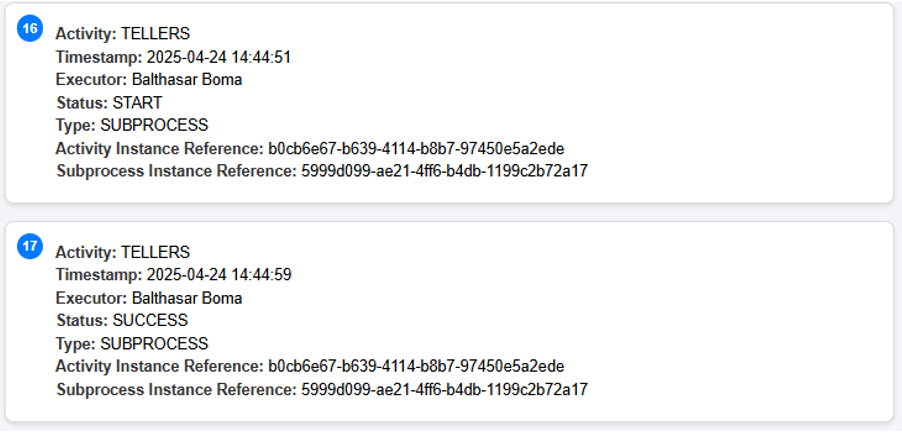
\includegraphics[width=1.0\linewidth]{subproces als activivty.png}
  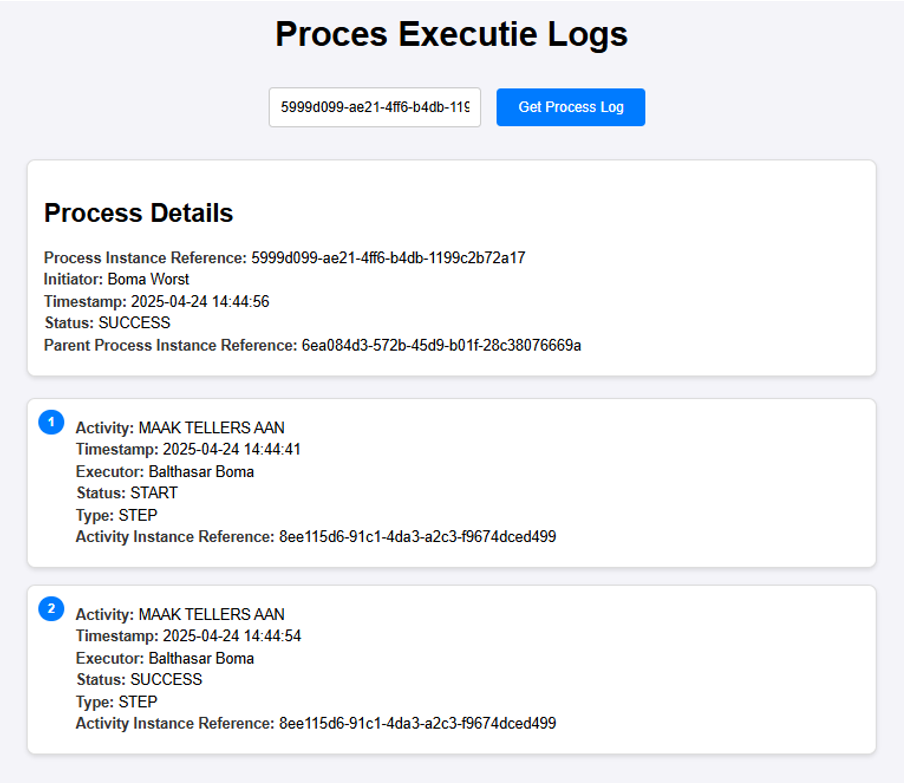
\includegraphics[width=1.0\linewidth]{subproces als log.png}
  \captionof{figure}[Subproces als traceerbare activiteit en executie log]{Het sub proces “TELLERS AANMAKEN” bestaat als zowel traceerbare activiteit instantie b0cb6e67-b639-4114-b8b7-97450e5a2ede als sub proces instantie 5999d099-ae21-4ff6-b4db-1199c2b72a17. Het sub proces kent zijn bovenliggende proces instantie 6ea084d3-572b-45d9-b01f-28c38076669a.}
\end{center}
 
Als volgens het proces er een taak dient genereerd te worden tijdens de activiteit, dan zal het systeem dit ook doen. Het zal deze taak ook slim uitdelen. Indien de monitoring aangeeft dat er iemand explicit bezig is aan een activiteit, dan zal de executie engine de taak genereren voor die specifieke medewerker zolang zijn werklast dit aankan. In elk ander geval zal het slim kijken naar de werklast van alle medewerkers en deze balanceren zodat iedereen evenveel taken heeft. \newline

De taken die te doen zijn kunnen opgehaald worden per medewerker om zo een takenoverzicht te maken voor de medewerker.

\begin{center}
  \captionsetup{type=figure}
  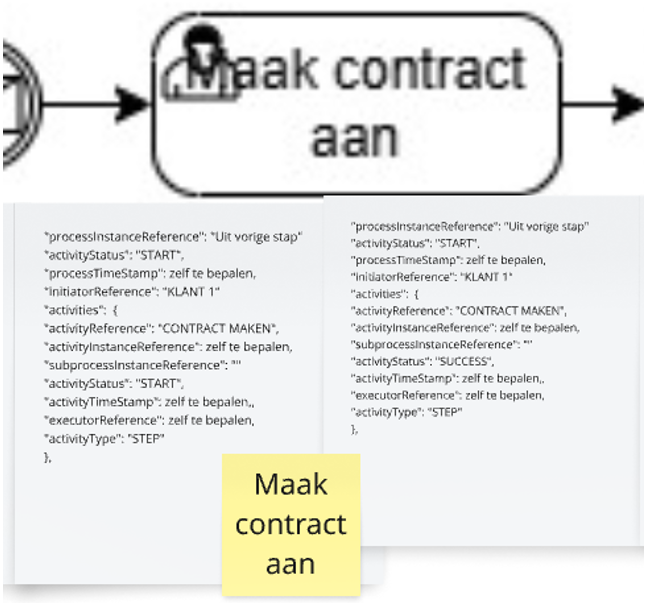
\includegraphics[width=1.0\linewidth]{bpmn taak ddt.png}
  \captionof{figure}[BPMN-diagram "contract maken" taak]{Het BPMN-diagram geeft aan dat activiteit “CONTRACT MAKEN” de taak “Maak contract aan” dient te genereren.}
\end{center}

\begin{center}
  \captionsetup{type=figure}
  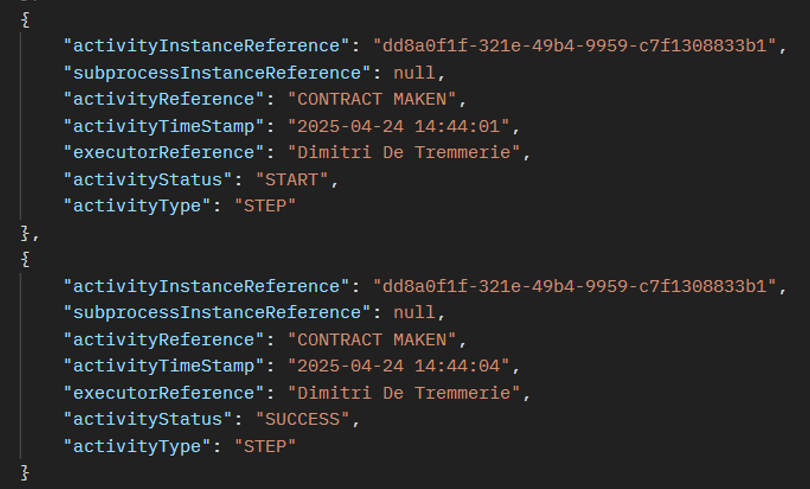
\includegraphics[width=1.0\linewidth]{json ddt.png}
  \captionof{figure}[JSON-output taak "contract maken" met toewijzing]{De monitoring gaf aan dat medewerker “Dimitri De Tremmerie” hieraan werkt.}
\end{center}

\begin{center}
  \captionsetup{type=figure}
  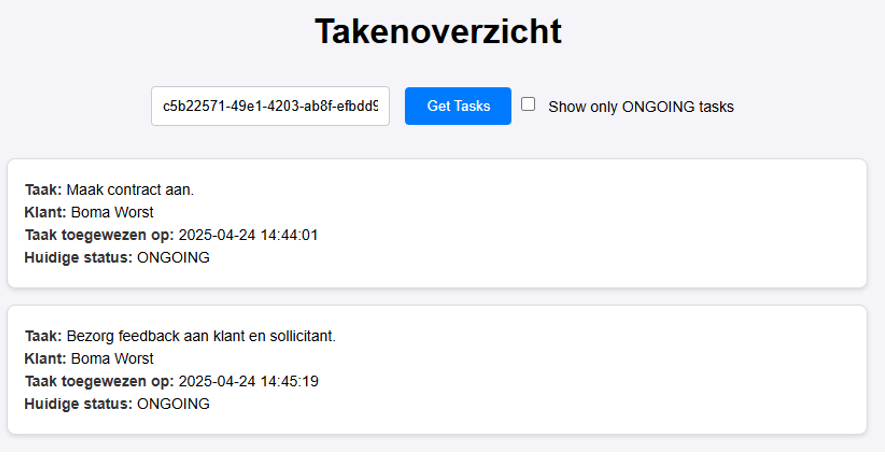
\includegraphics[width=1.0\linewidth]{visualisatie ddt.png}
  \captionof{figure}[Visualisatie taak "contract maken" met toewijzing]{De taak wordt expliciet gemaakt voor deze medewerker en komt in zijn overzicht op hetzelfde moment.}
\end{center}

\begin{center}
  \captionsetup{type=figure}
  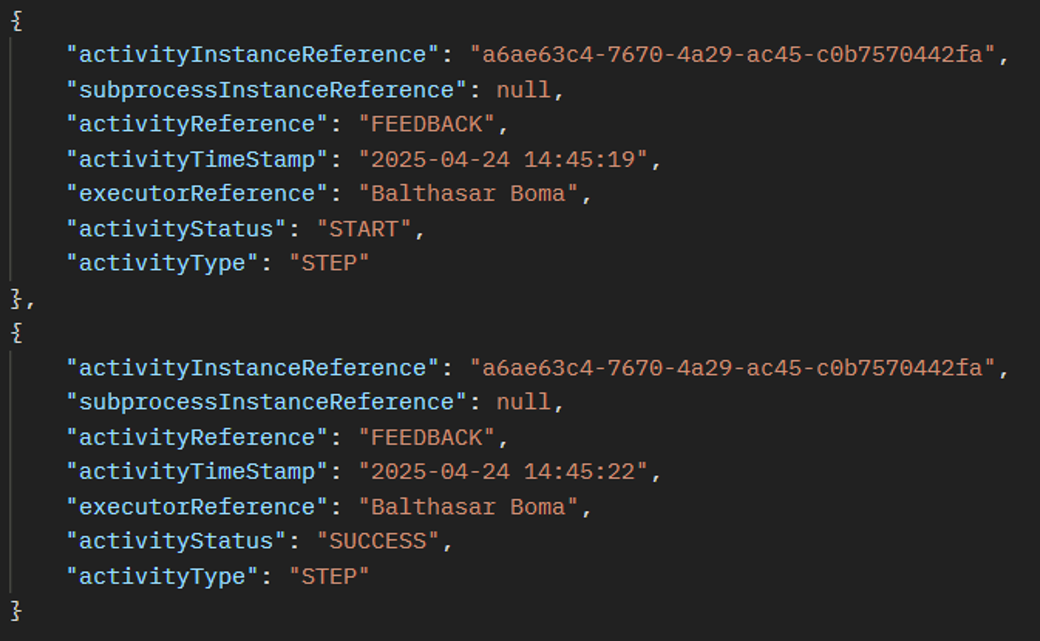
\includegraphics[width=0.75\linewidth]{log boma.png}
  \captionof{figure}[JSON-output slimme toewijzing taken]{De tweede taak uit vorige screenshot was eerst volgens de monitoring voor medewerker “Balthasar Boma”, maar de executie engine nam dit uit zijn handen omdat deze over zijn takenlimiet zou zitten.}
\end{center}

Indien het systeem bevestiging krijgt dat een taak voltooid of gefaald is, dan is deze uit het overzicht te filteren.
 
\begin{center}
  \captionsetup{type=figure}
  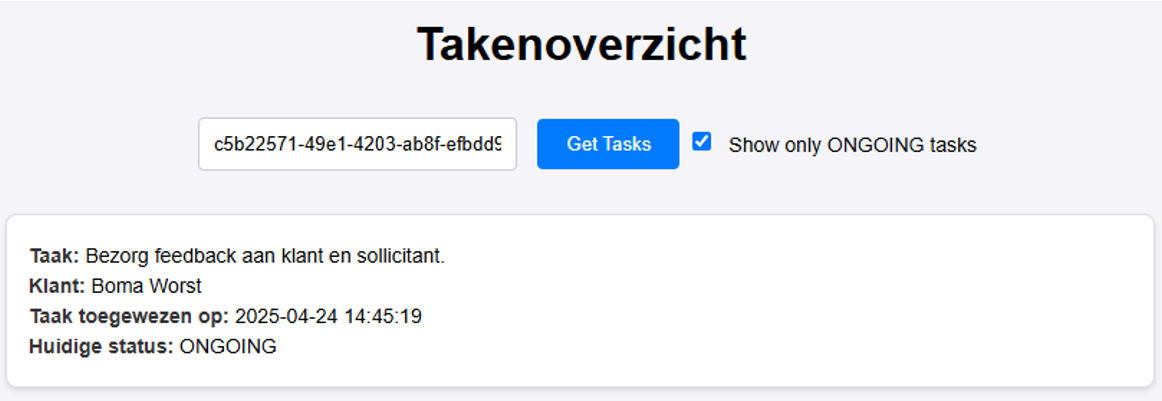
\includegraphics[width=1.0\linewidth]{takenoverzicht filtered.png}
  \captionof{figure}[Visualisatie takenoverzicht met filtering]{Het takenoverzicht met filtering op doorlopende taken.}
\end{center}

Het systeem registreert echter wel de status en moment van beëindiging. Gezien elke type taak via zijn taak referentie traceerbaar blijft, kan zo aan statistisch onderzoek en anomaliedetectie gedaan worden.
 
\begin{center}
  \captionsetup{type=figure}
  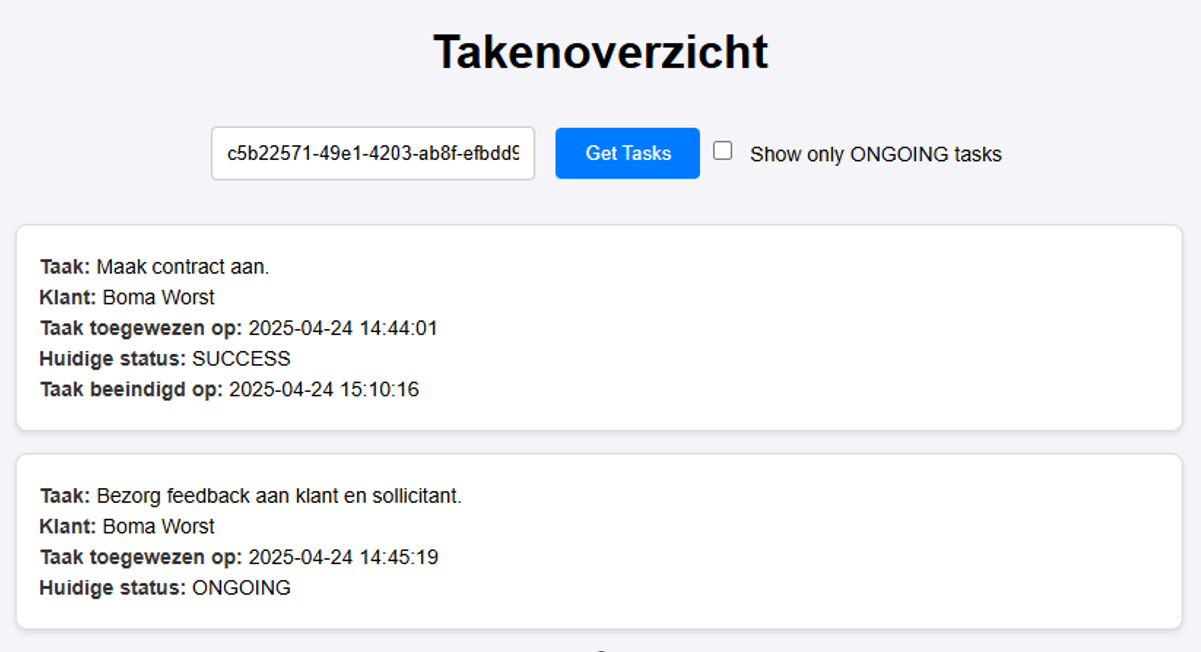
\includegraphics[width=1.0\linewidth]{takenoverzicht non-filtered.png}
  \captionof{figure}[Visualisatie takenoverzicht zonder filtering]{Het takenoverzicht met voltooide taken voor statistisch onderzoek en anomaliedetectie.}
\end{center}